%%%%%%%%%%%%%%%%%%%%%%%%%%%%%%%%%%%%%%%%%%%%%%%%%%%%%%%%%%%%%%%%%%%%%%%%
%%%  THIS TEX FILE IS TO GENERATE PDF FILE FOR 
%%% 
%%%  COPYRIGHT (C) JIMMY LIN, 2013, UT AUSTIN
%%%%%%%%%%%%%%%%%%%%%%%%%%%%%%%%%%%%%%%%%%%%%%%%%%%%%%%%%%%%%%%%%%%%%%%%
\documentclass[10pt]{beamer}
%%%%%%%%%%%%%%%%%%%%%%%%%%%%%%%%%%%%%%%%%%%%%%%%%%%%%%%%%%%%%%%%%%%%%%%%
%%%  PACKAGES USED IN THIS TEX SOURCE FILE
%%%%%%%%%%%%%%%%%%%%%%%%%%%%%%%%%%%%%%%%%%%%%%%%%%%%%%%%%%%%%%%%%%%%%%%%
\usepackage{graphicx}
\usepackage{wrapfig}
\usepackage{geometry}
\usepackage{color}
\usepackage{JSPPT}
\usepackage[style=ieee]{biblatex}
%%%%%%%%%%%%%%%%%%%%%%%%%%%%%%%%%%%%%%%%%%%%%%%%%%%%%%%%%%%%%%%%%%%%%%%%
%%% PRESENTATION INFORMATION
%%%%%%%%%%%%%%%%%%%%%%%%%%%%%%%%%%%%%%%%%%%%%%%%%%%%%%%%%%%%%%%%%%%%%%%%
\title{Multiagent Behaviors in Neural Network}
\author[Jimmy Lin and Barry Feigenbaum]{\bf Jimmy Lin \\Barry Feigenbaum}
\institute{\bf Prof. Risto Miikkulainen\\[0.3cm] Department of Computer Science \\The University of Texas At Austin}

%%%%%%%%%%%%%%%%%%%%%%%%%%%%%%%%%%%%%%%%%%%%%%%%%%%%%%%%%%%%%%%%%%%%%%%%
%%% TITLE PAGE
%%%%%%%%%%%%%%%%%%%%%%%%%%%%%%%%%%%%%%%%%%%%%%%%%%%%%%%%%%%%%%%%%%%%%%%%
\begin{document}
\begin{large}
    \frame{\maketitle}%\titlepage
\end{large}

\frame{
    \frametitle{Table of Contents}
    \tableofcontents
}

%%%%%%%%%%%%%%%%%%%%%%%%%%%%%%%%%%%%%%%%%%%%%%%%%%%%%%%%%%%%%%%%%%%%%%%%
%%% DOCUMENTATION STARTS FROM HERE
%%%%%%%%%%%%%%%%%%%%%%%%%%%%%%%%%%%%%%%%%%%%%%%%%%%%%%%%%%%%%%%%%%%%%%%%
\section{Overview of Multiagent System}
\setbeamertemplate{itemize item}[ball]
\setbeamertemplate{itemize subitem}{$\int$}
% recapture contents of previous topic talks
\frame{
    \frametitle{Recap}
        What we currently have? 
            \begin{itemize}
                \item Commitee Machine 
                \item Reinforcement Learning
                \item Neuro-evolution
                \item High-level Behaviors
            \end{itemize}
}
\frame{
    \frametitle{Motivation}
    \begin{itemize}
        \item Most of works so far has focused exclusively on single agents
            we can extend reinforcement learning straightforwardly to multiple
            agents if they are all independent. 
        \item Intuitive idea: Multiple agents together will outperform
            any single agent due to the fact that they have more resources and
            a better chance of receiving rewards.
        \item Today, we will touch a really broad area 
            $$ \text{"Multiagent System" (M.A.S.).}
            $$
    \end{itemize}
}
% introduce multiagent behavior
\frame{
    \frametitle{Introduction}
         What is multiple agent system?
            \begin{itemize}
                \item Unfortunately, it is not formally defined by M.A.S. community.
                \item Employment of multiple agents (10 to thousands). 
                \item Intelligent mechanisms to address interactions between
                    agents.
            \end{itemize}
         When is it proposed?
            \begin{itemize}
                \item a relatively new sub-field of computer science 
                \item has only been studied since about 1980
                \item only gained widespread recognition since
                    about the mid-1990s
            \end{itemize}
}
\frame{
    \frametitle{M.A.S. Environments}
    The agents in a multi-agent system have several important characteristics:
    \begin{itemize}
        \item Autonomy: the agents are at least partially independent, self-aware, autonomous.
        \item Local views: no agent has a full global view of the system, or
            the system is too complex for an agent to make practical use of
            such knowledge.
        \item Decentralization: there is no designated controlling agent (or
            the system is effectively reduced to a monolithic system).
    \end{itemize}
}
\frame{
    \frametitle{Applications/Simulations}
    \begin{itemize}
        \item Pacman
        \item
            \href{https://www.youtube.com/watch?v=pqBSNAOsMDc&index=12&list=PLD56A0C7765234DCD}{Crowd
                Simulation / Crowd Collision Avoidance}
        \item    \href{https://www.youtube.com/watch?v=Hc6kng5A8lQ&index=13&list=PLD56A0C7765234DCD}
            {ClearPath: Highly Parallel Collision Avoidance for Multi-agent Simulation}
        \item \href{https://www.youtube.com/watch?v=azIOCFjDZWA&list=PL5Tiw7DXCdu2roBlpHvUzOMvR7WGXMoP6}{MATISSE: A Multi-Agent based Traffic Simulation System}
    \end{itemize}
}
% 
\frame{
    \frametitle{Independent v.s. Cooperative Agents}
     Tang Ming (1993) \cite{1} studied the performance of cooperative agents,
     using independent agents as a benchmark. Here are the discoveries:
    \begin{itemize}
        \item Additional sensation from another agent is beneficial if it can
            be used efficiently.
        \item Sharing learned policies or episodes among agents speeds up
            learning at the cost of communication.
        \item For joint tasks, agents engaging in partnership can
            significantly outperform independent agents although they may
            learn slowly in the beginning.
    \end{itemize}
}

\frame{
    \frametitle{Active Research Areas}
    Currently active research areas of M.A.S. are advanced Multiagent
    Behaviors, as follows:
    \begin{itemize}
        \item Communication
        \item Cooperation and Coordination
        \item Negotiation
        \item Distributed Problem Solving
        \item Multi-agent Learning
        \item Fault Tolerance
    \end{itemize}
}
% explain each multiagent behavior
\frame{
    \frametitle{Communication}
    {\bf Communication} is defined as altering the state of the environment
    such that other agents can perceive the modification and decode
    information from it.
    \begin{itemize}
        \item Direct Communication
        \item Indirect Communication
    \end{itemize}
}
\frame{
    \frametitle{Cooperation and Coordination}
}
\frame{
    \frametitle{Negotiation}
}
\frame{
    \frametitle{Distributed Problem Solving}
    The state space of a large, joint multi-agent task can be overwhelming. An obvious way to tackle this is to use domain
knowledge to simplify the state space, often by providing a smaller set of
more “powerful” actions customized for the problem domain. 

An alternative has been to reduce complexity
by heuristically decomposing the problem, and hence the joint behavior, into
separate, simpler behaviors for the agents to learn. Such decomposition may be
done at various levels (decomposing team behaviors into sub-behaviors for each
agent; decomposing an agents’ behavior into sub-behaviors; etc.), and the
behaviors may be learned independently, iteratively (each depending on the
earlier one), or in a bottom-up fashion (learning simple behaviors, then
grouping into “complex” behaviors).
}
\frame{
    \frametitle{Multi-agent Learning}
}
\frame{
    \frametitle{Fault Tolerance}
}
%%%%%%%%%%%%%%%%%%%%%%%%%%%%%%%%%%%%%%%%%%%%%%%%%%%%%%%%%%%%%%%%%%%%%%%%
\section{Detailed Research Literature}

\frame{
    \frametitle{Social Learning}
    \begin{columns}[T] 
             \begin{column}[T]{5cm} 
             \begin{itemize}
                 \item In \textbf{social learning}, agents improve their own performance by learning from observations made by other members of the population
                 \item Traditionally, agents are partitioned into students and teachers, where teachers are chosen to be high fitness members of the population
                 \item \textbf{Problem}: Fitness is not a guarantee of superior behavior. High fitness agents may make mistakes, and low fitness agents can still do well under certain circumstances
                 \end{itemize}
             \end{column}
             \begin{column}[T]{4cm} 
             	
\includegraphics[width=4.5cm]{images/social_learning.png}
             \end{column}
        \end{columns}
}

\frame{
    \frametitle{Cooperative search}
    \begin{columns}[T] 
             \begin{column}[T]{4cm} 
             \begin{itemize}
                \item In this example, agents represent \textbf{Unmanned Aerial Vehicles} (\textbf{UAVs}) searching a grid of airspace 
                \item Agents have limited communication and some mobility restrictions (such as slow turning)
             \end{itemize}
             \end{column}
             \begin{column}[T]{6.5cm} 
             	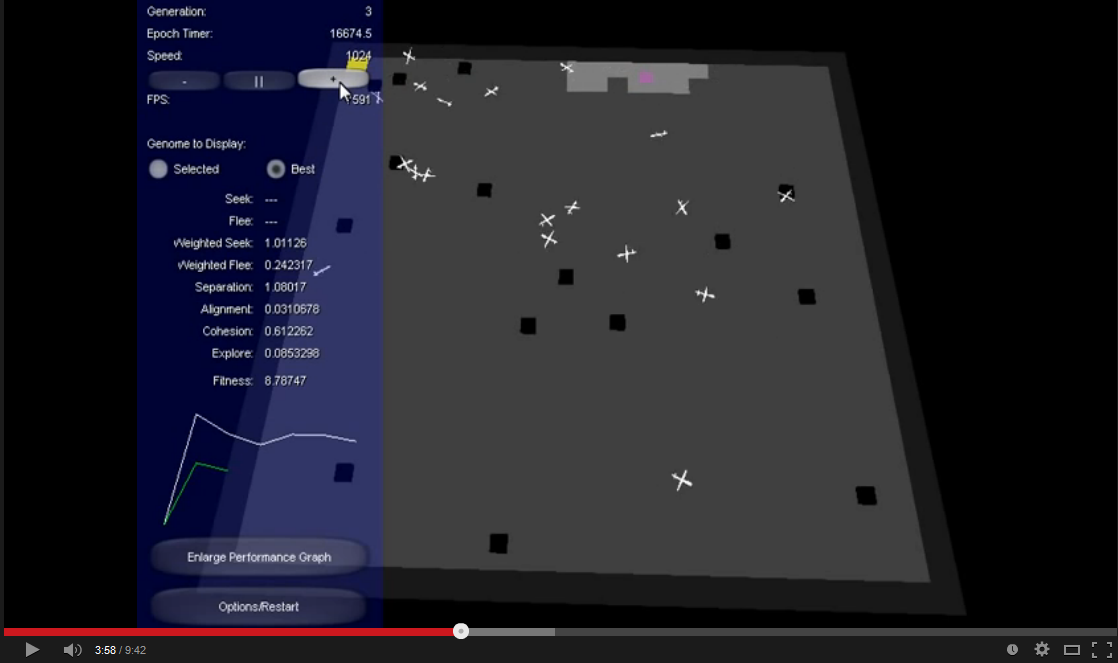
\includegraphics[width=7cm]{images/uav/youtube.png}
             \end{column}
        \end{columns}
}

\frame{
    \frametitle{UAV Example: Goals}
    \begin{columns}[T] % contents are top vertically aligned
         \begin{column}[T]{5cm} % each column can also be its own environment
         \begin{itemize}
             \item Compare a \textit{centralized} approach, where agents share a network, to a \textit{decentralized} approach
             \item Determine whether opportunistic sharing of network weights improves the speed and accuracy of learning
         \end{itemize}
         \end{column}
         \begin{column}[T]{6cm} % alternative top-align that's better for graphics
              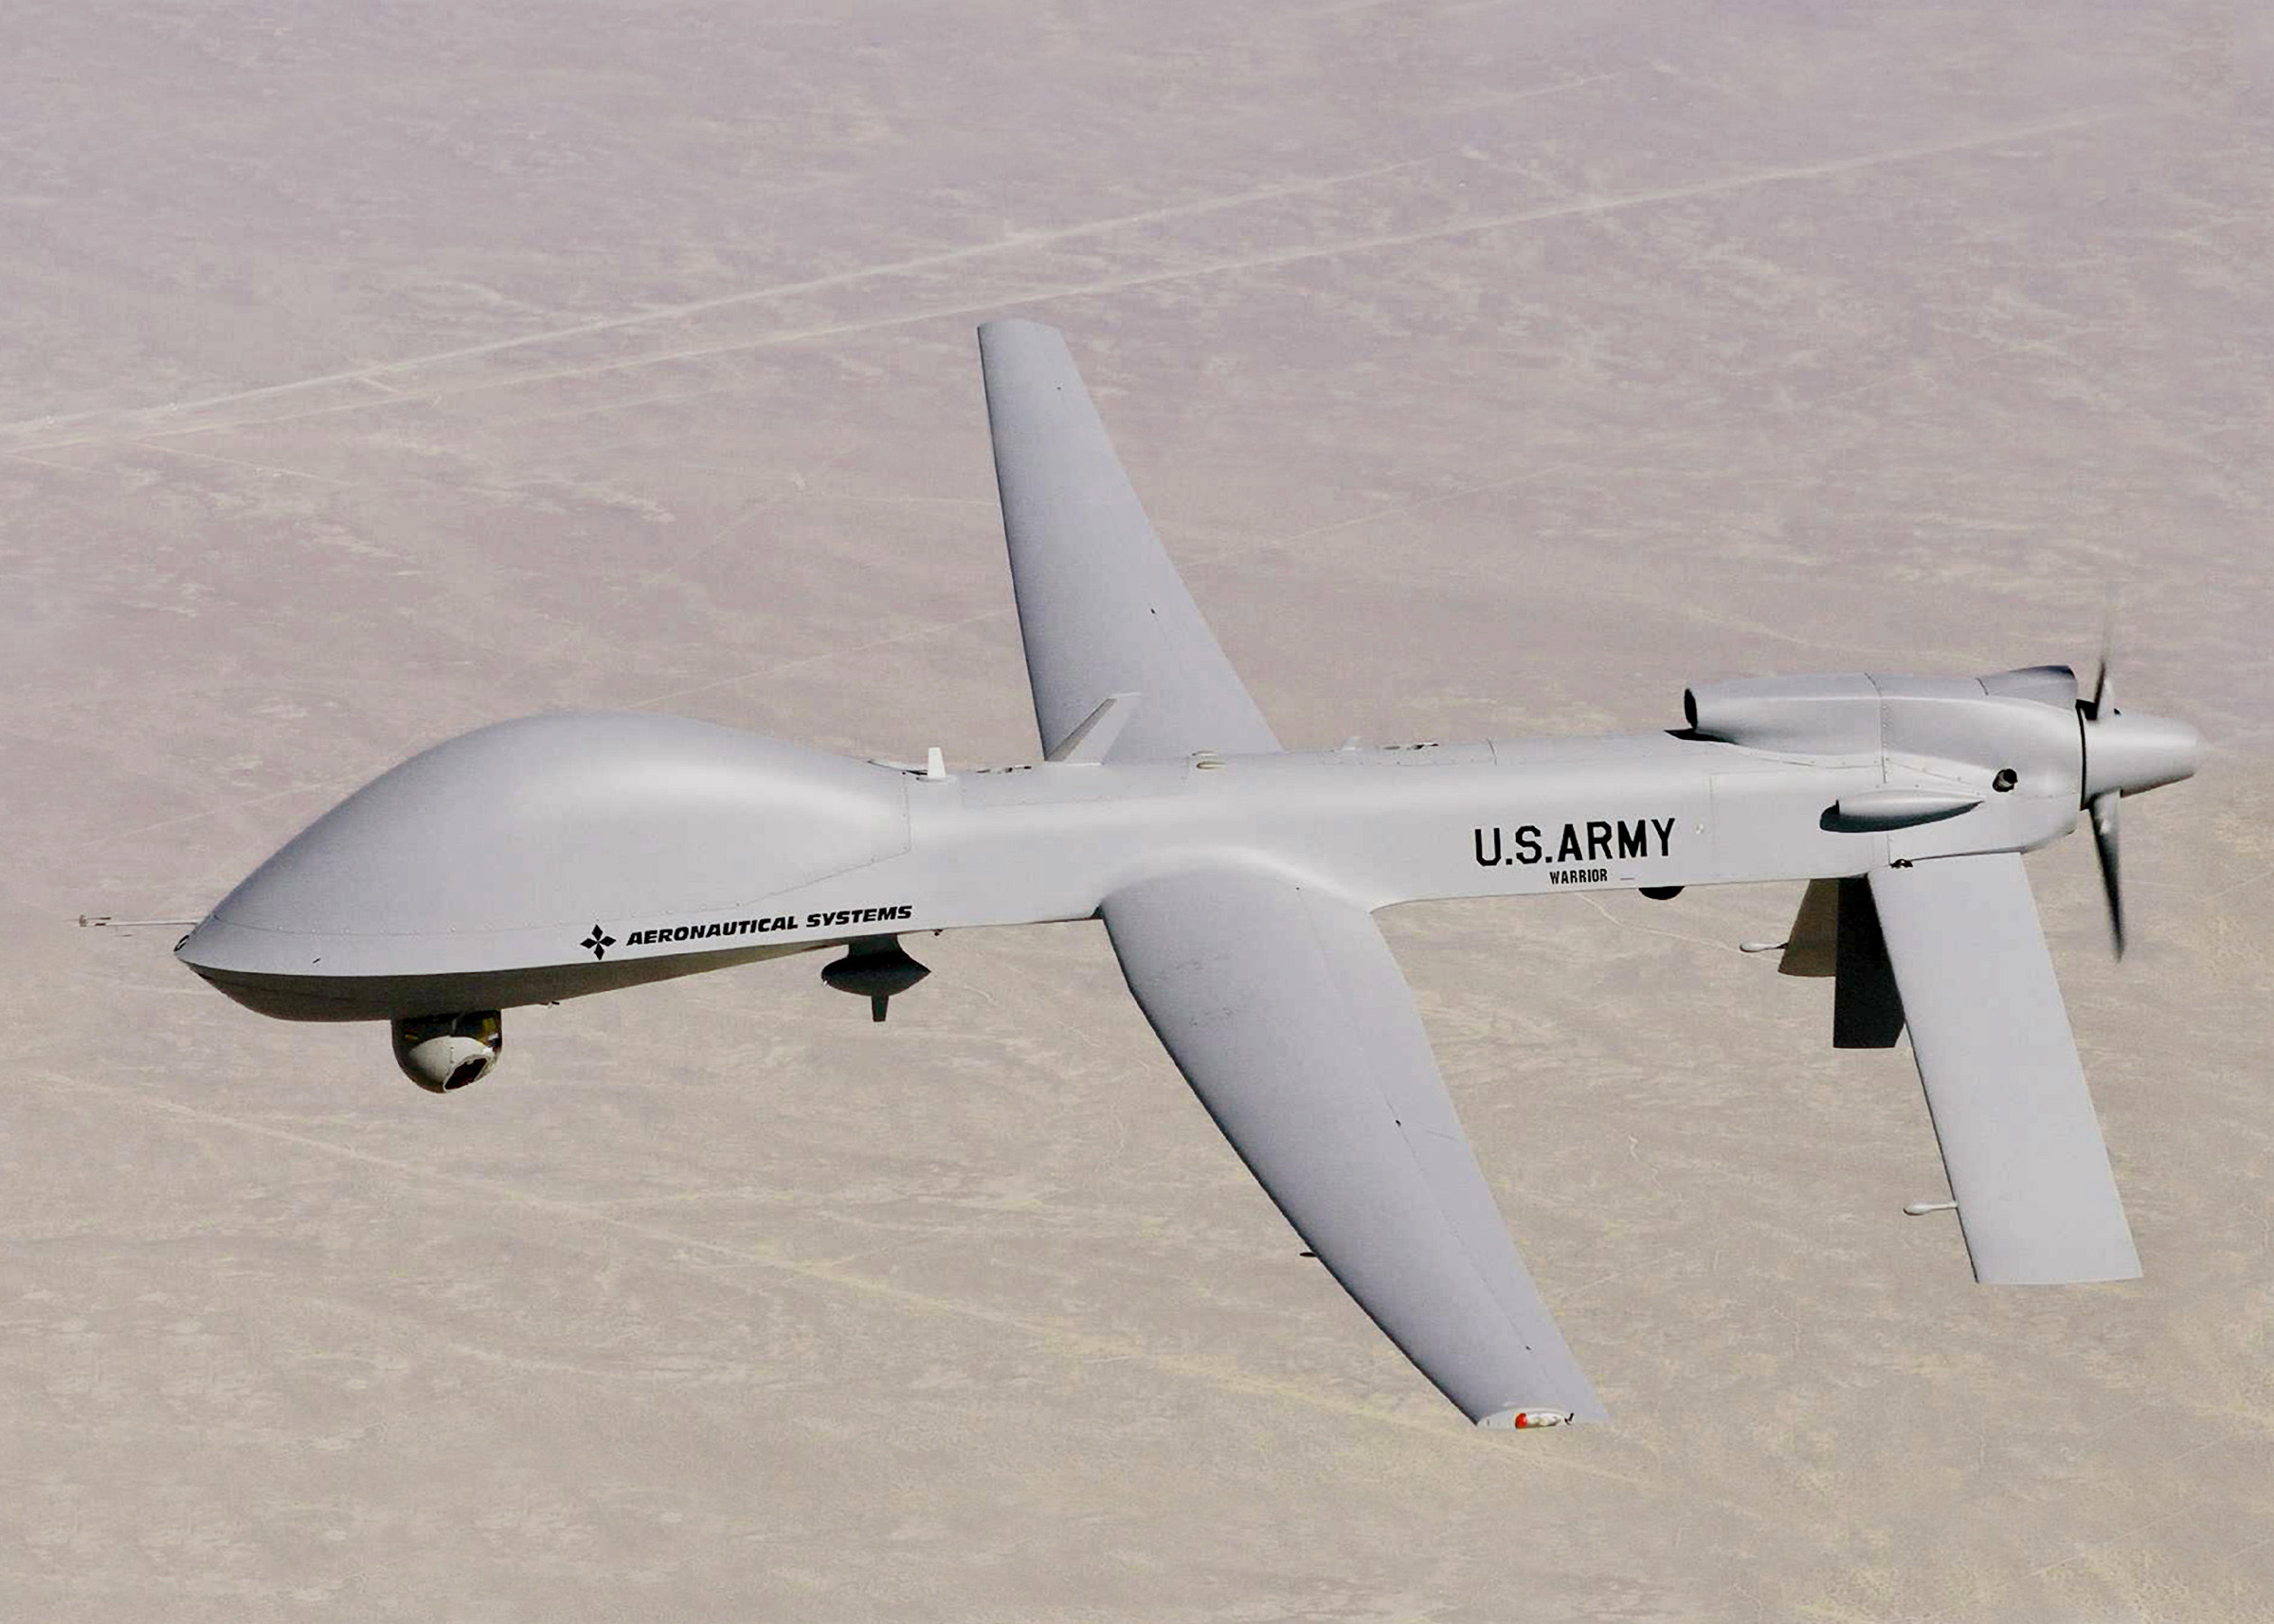
\includegraphics[width=6cm]{images/uav/UAV_Drone.jpg}
         \end{column}
    \end{columns}
    
}

\frame{
    \frametitle{UAV Example: Setup}
    \begin{columns}[T] 
    	\begin{column}[T]{5cm} 
		    \begin{itemize}
		    \item Trained via Reinforcement Learning
		    \item The search space is divided into a grid, and each cell is given a \textit{certainty} value between 0 and 1 
		    \item The uncertainty of a cell is reduced by half for each agent that enters that cell
		    \item Rewards equal the decrease in uncertainty in a given cell divided evenly among the entering agents 
		    \end{itemize}
		\end{column}
		\begin{column}[T]{5cm}
			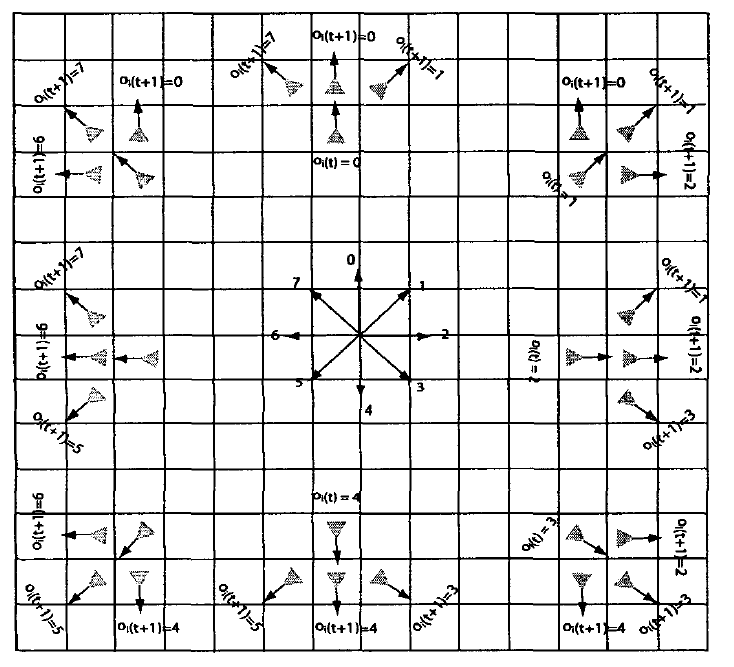
\includegraphics[width=5.5cm]{images/uav/overview.png}
		\end{column}
	\end{columns}
}

\frame{
    \frametitle{UAV Example}
    \begin{itemize}
    \item Agents want to spread out and avoid entering the same cell
    \item At each time-step, an agent only has three options (turn left, turn right, keep straight)
    \item Three neural networks are used to estimate the benefit of each course
    \end{itemize}
    Compare three architectures:
	\begin{itemize}
	\item \textbf{Centralized Learning}: three shared networks receive input from all agents
	\item \textbf{Decentralized Learning}: each agent has it's own three networks
	\item \textbf{Opportunistic Cooperative Learning}: each agent has it's own three networks. Additionally, when two agents come close together, the less successful one copies the other's network with probability $\pi$
	\end{itemize}
}

\frame{
    \frametitle{UAV Example: Results}
    \begin{center}
    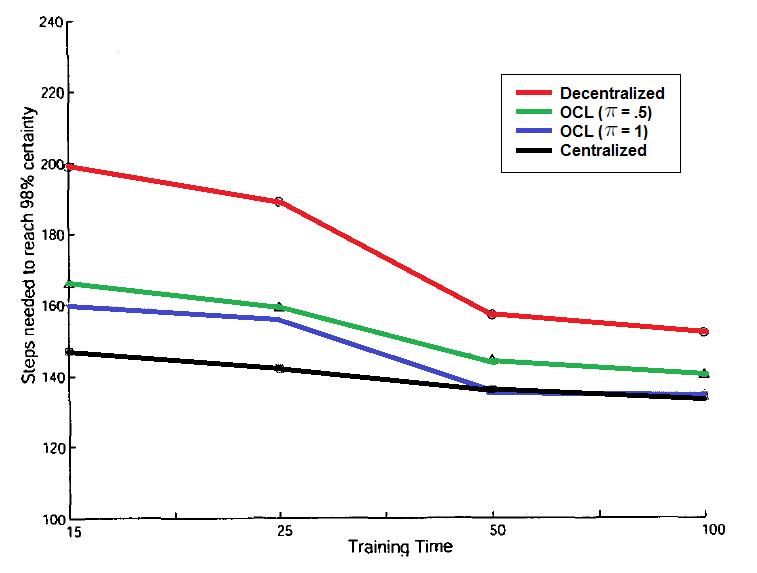
\includegraphics[height=7cm]{images/uav/results_color.png}
    \end{center}
    
}

\frame{
    \frametitle{Egaltarian Social Learning}
    \begin{itemize}
    \item In \textbf{Egaltarian Social Learning} (\textbf{ESL}), agents learn from each other instead of from a limited number of teachers 
    \item The population of agents is partitioned into subcultures at the start of each generation
    \item An agent may probabilistically learn from any other agent in the same subculture
    %\item An agent's quality as an example is determined by the receiving agent
    \end{itemize}
}

\frame{
    \frametitle{ESL Example: Foraging}
    \begin{itemize}
    \item Agents move independently across a continuous world filled with several types of plants
    \item Plants are automatically consumed when an agent draws close enough; some types of plant give positive reward, others negative reward
    \item Agents have sensors for each type of plant, as well as a sensor for their own velocity
    \item They cannot see other agents, or plants they have already consumed
    \item Networks are trained with backpropagation and NeuroEvolution of Augmenting Topologies (NEAT)
    \end{itemize}
}

\frame{
    \frametitle{ESL Example: Foraging (Results)}
    \begin{columns}[T] % contents are top vertically aligned
         \begin{column}[T]{4cm} % each column can also be its own environment
         \begin{itemize}
             \item ESL without subcultures performs worse than plain neuroevolution
             \item Adding subcultures results in a significant improvement
         \end{itemize}
         \end{column}
         \begin{column}[T]{6cm} % alternative top-align that's better for graphics
              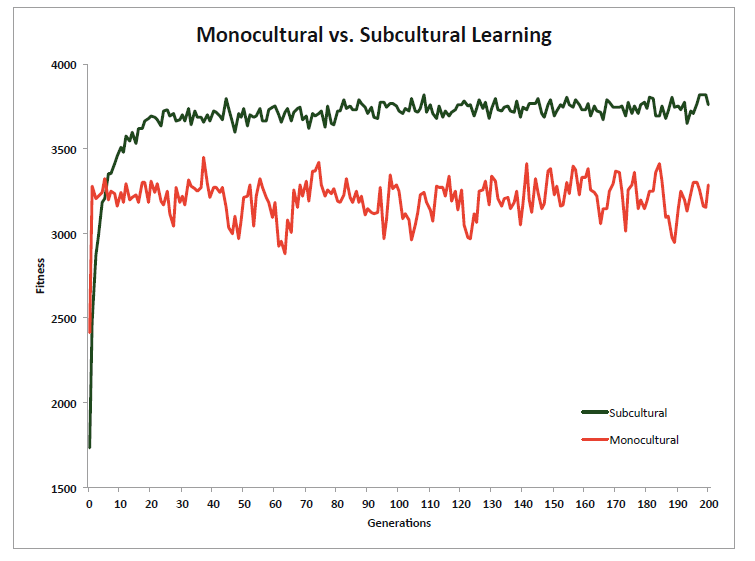
\includegraphics[height=5cm]{images/foraging/monocultural_vs_subcultural.png}
         \end{column}
    \end{columns}
    
}

\frame{
    \frametitle{ESL Example: Foraging (Results)}
    Comparing ESL with student-teacher learning and plain neuroevolution
    \begin{columns}[T] 
         \begin{column}[T]{4.5cm} 
         	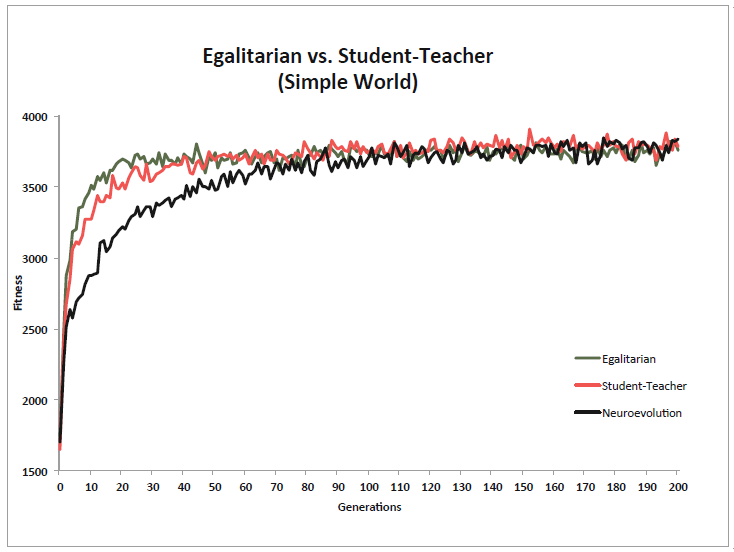
\includegraphics[height=4.2cm]{images/foraging/student_teacher_simple.png}
         	
         	Simple environment (few plant types)
         \end{column}
         \begin{column}[T]{4.5cm} 
           	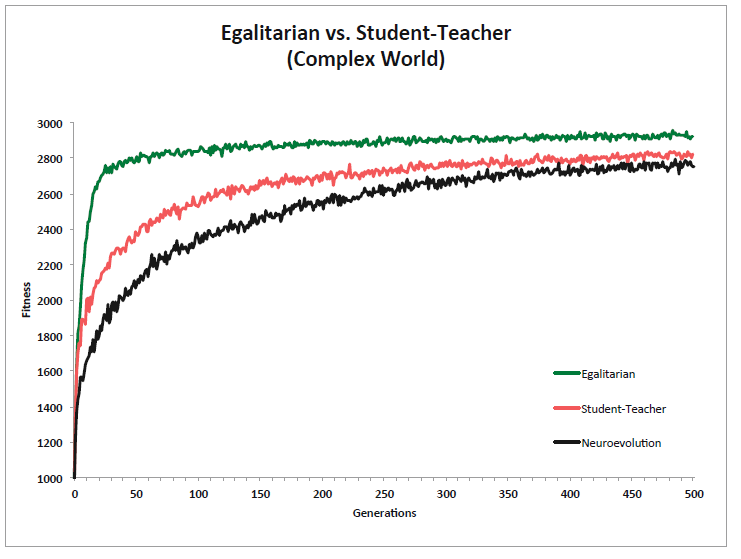
\includegraphics[height=4.2cm]{images/foraging/student_teacher_complex.png}
           	
           	Complex environment (many plant types)
         \end{column}
    \end{columns}
}

\frame{
    \frametitle{ESL Example: Foraging (Conclusion)}
    \begin{itemize}
    \item ESL is advantageous because it promotes diversity and avoids premature convergence
    \end{itemize}
}

\frame{
    \frametitle{Communication}
     
}

\frame{
    \frametitle{Predator / Prey}
    \begin{columns}[T] 
        \begin{column}[T]{5cm}
			Three different examples:
		  	\begin{itemize}
		  	\item Centralized network
		  	\item Autonomous networks with communication
		  	\item Autonomous networks \textit{without} communication
		  	\end{itemize}
		  	All are trained using ESP or \textbf{Multi-Agent ESP} 
	  	\end{column}
	  	\begin{column}[T]{6cm}
			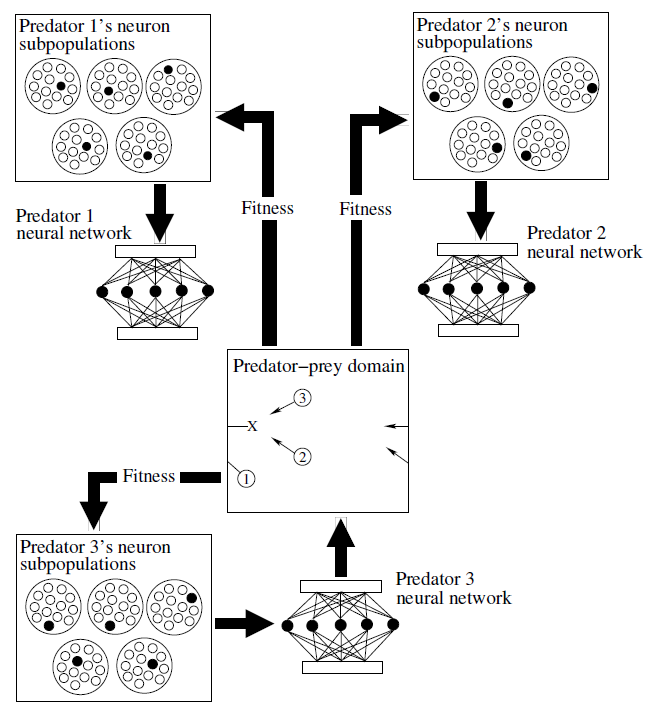
\includegraphics[width=5.5cm]{images/predator_prey/multiagent_esp.png}
	  	\end{column}
	\end{columns}
}

\frame{
    \frametitle{Centralized Network}
    \begin{center}
    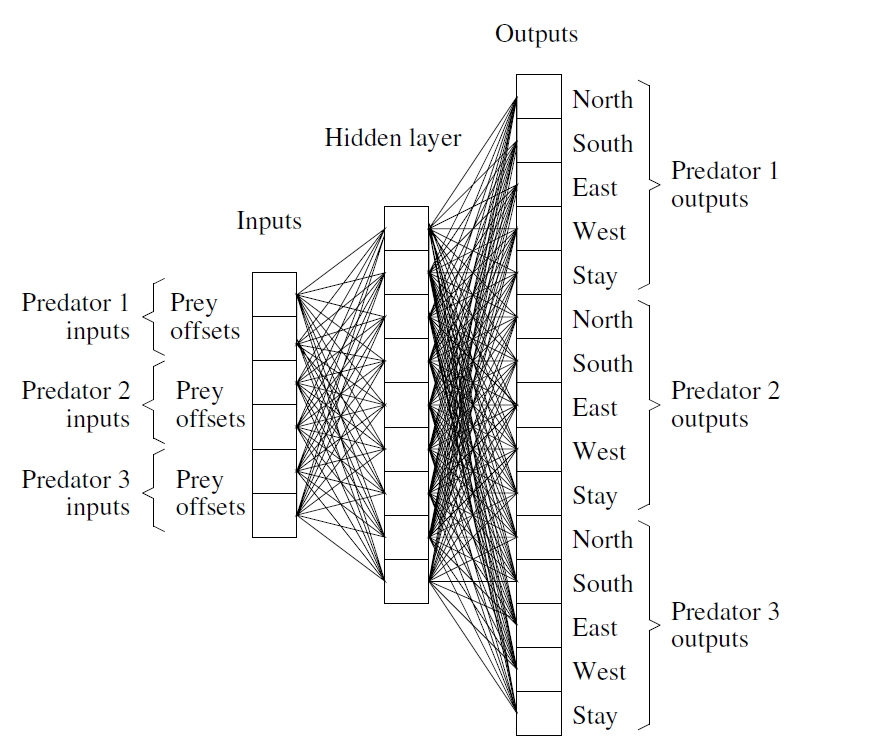
\includegraphics[width=9cm]{images/predator_prey/central_network.png}
    \end{center}
}

\frame{
    \frametitle{Communicating Network}
    \begin{center}
    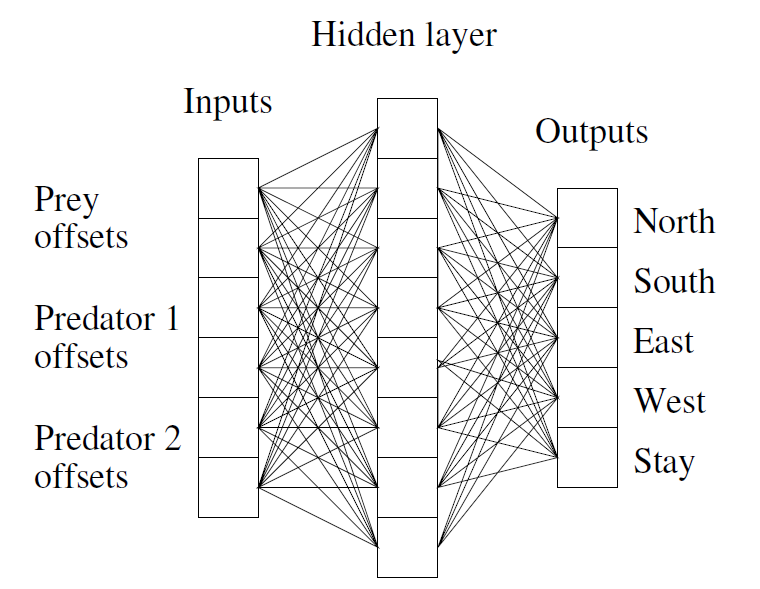
\includegraphics[width=8cm]{images/predator_prey/communication_network.png}
    \end{center}
}

\frame{
    \frametitle{Non-communicating Network}
    \begin{center}
    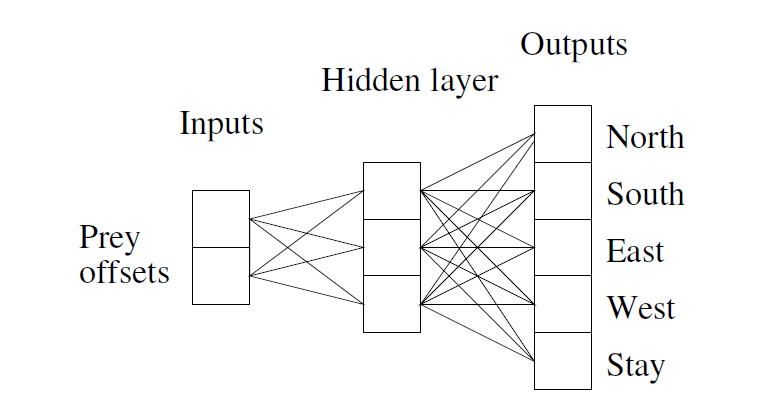
\includegraphics[width=8cm]{images/predator_prey/noncommunication_network.png}
    \end{center}
}

\frame{
    \frametitle{Predator / Prey Results}
    How long does it take these networks to become successful?
    \begin{columns}[T] 
         \begin{column}[T]{6cm} 
         	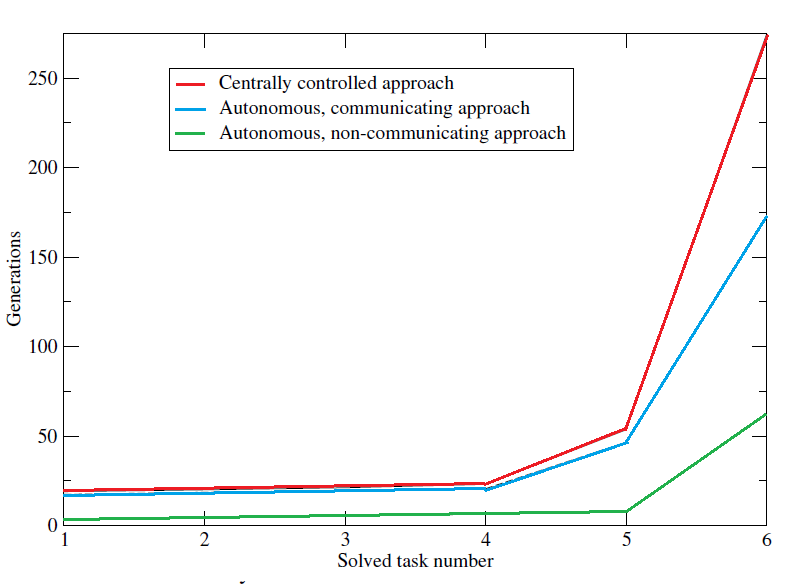
\includegraphics[height=4.5cm]{images/predator_prey/results_line.png}
         	\begin{center}
         	\end{center}
         \end{column}
         \begin{column}[T]{6cm} 
           	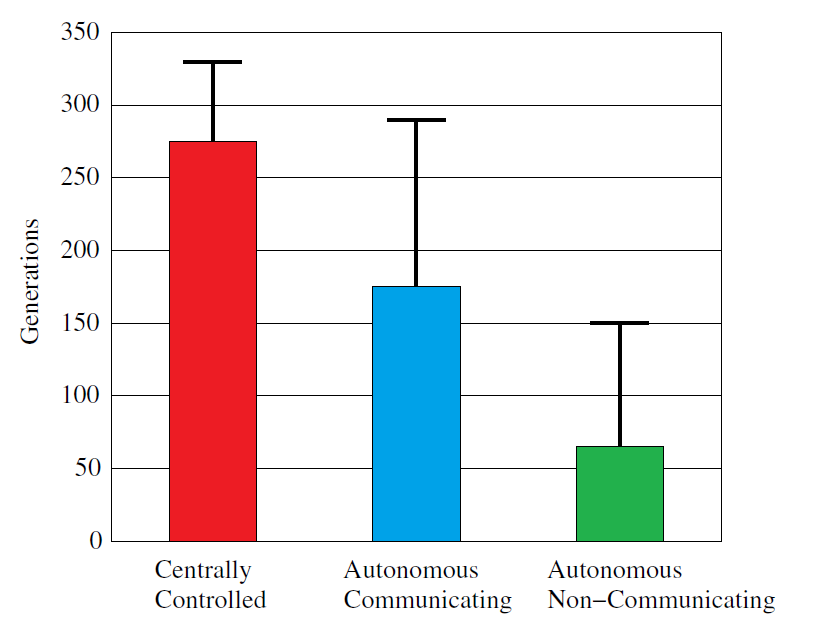
\includegraphics[height=4.5cm]{images/predator_prey/results_bar.png}
           	\begin{center}
           	\end{center}
         \end{column}
    \end{columns}
    \textbf{Conclusion}: The predators are able to cooperate using \textbf{stigmergy} -- indirect coordination based on the environment
    \begin{itemize}
    \item What if the environment is more complicated?
    \end{itemize}  
}

\frame{
    \frametitle{Predator / Prey Conclusion}
    \begin{itemize}
    \item What happens if we use homogeneous networks? (All predators have the same network weights)
    \item Communication becomes a necessity
    \end{itemize}
    \begin{center}
    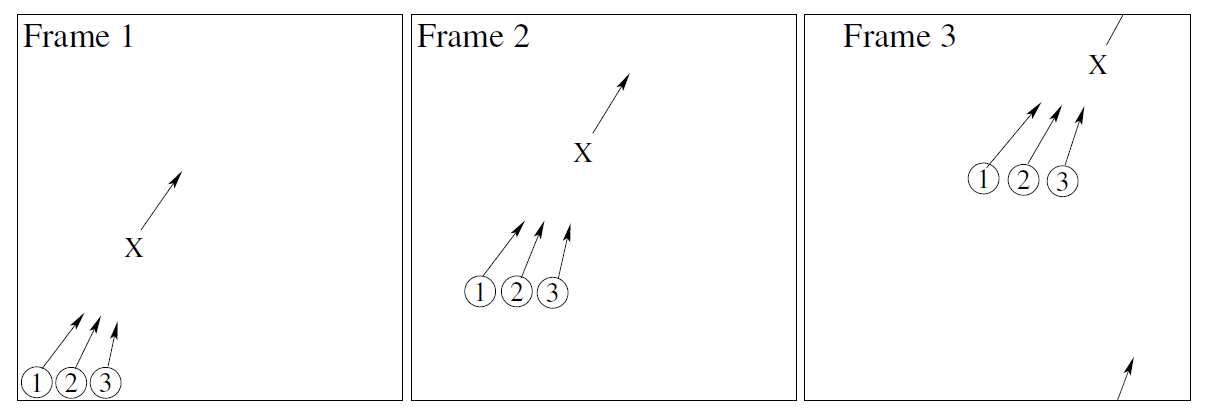
\includegraphics[width=9cm]{images/predator_prey/no_cooperation.png} 
    \end{center}
    \begin{itemize}
    \item Even with communication, homogeneous networks do poorly, catching the prey only 3\% of the time
    \end{itemize} 
}

\frame{
    \frametitle{Homogeneous Networks}
    \begin{itemize}
    \item Thus far, all multi-agent solutions have used heterogeneous networks
    \item In the predator prey, homogeneous networks performed very poorly
    \item Can we evolve agents with identical networks, which nevertheless cooperate by adopting different strategies?
    \end{itemize}
}

\frame{
    \frametitle{Legion Game}
    \begin{columns}[T] 
         \begin{column}[T]{4cm} 
         	The Legion game consists of:
         	\begin{itemize}
         	\item A hexagonal grid (the countryside)
         	\item A number of randomly placed cities
         	\item Several legions (defenders)
         	\item Many barbarian attackers
         	\end{itemize}
         	At every game tick, legions are penalized for each barbarian on the board
         \end{column}
         \begin{column}[T]{7cm} 
           	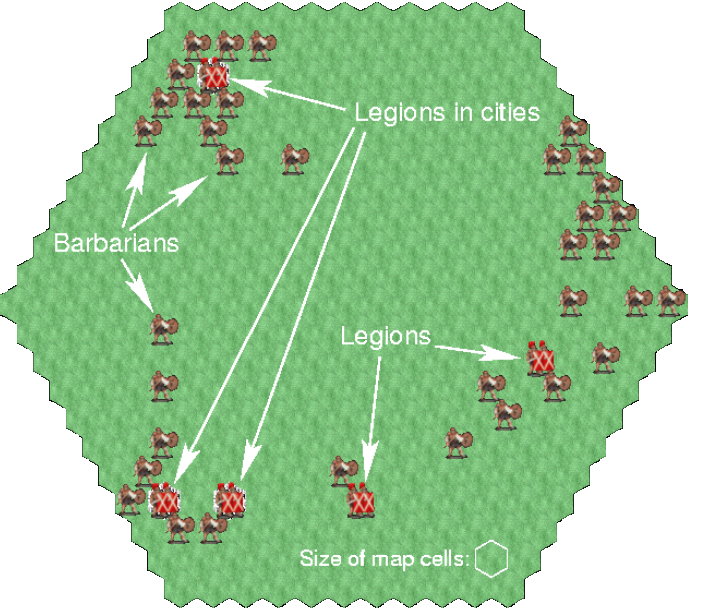
\includegraphics[height=6cm]{images/legion/setup.png}
         \end{column}
    \end{columns}
}

\frame{
    \frametitle{Legion Network}
    \begin{itemize}
    \item Each legion has six sensors for each of the six directions
    \item Can detect immediate adjacency as well as long-distance
    \end{itemize}
    \begin{columns}[T] 
         \begin{column}[T]{5.5cm} 
         	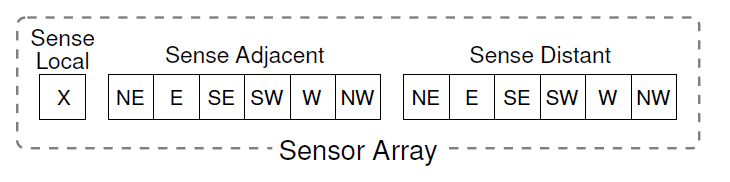
\includegraphics[width=6cm]{images/legion/inputs.png}
         	
         	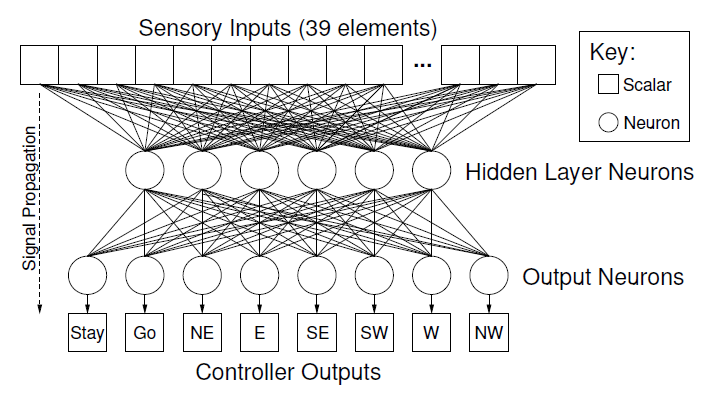
\includegraphics[width=6cm]{images/legion/network.png}
         \end{column}
         \begin{column}[T]{4.5cm} 
           	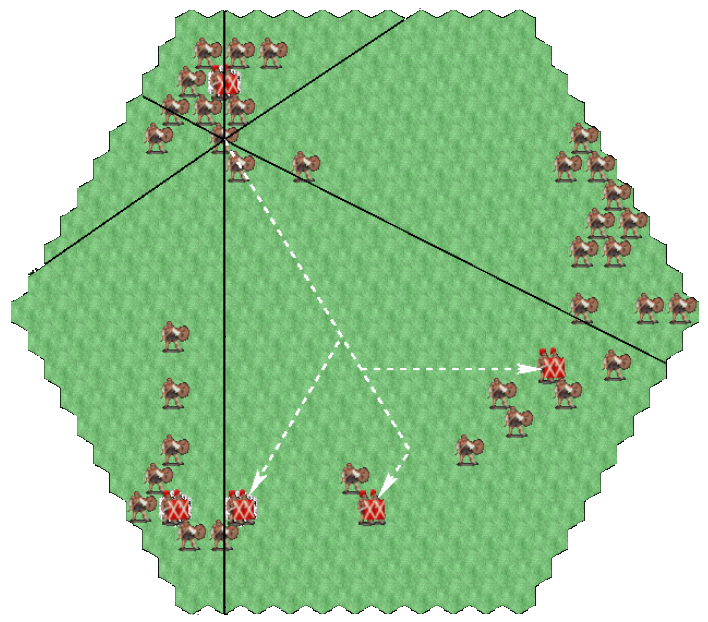
\includegraphics[width=5cm]{images/legion/sensors.png}
         \end{column}
    \end{columns}
}

\frame{
    \frametitle{Legion Results}
    \begin{itemize}
    \item Legions were trained with ESP neuroevolution
    \item Successfully learned to divide labor between "guard duty" and search and destroy" behavior
    \end{itemize}
    
    \begin{columns}[T] 
         \begin{column}[T]{5cm} 
         	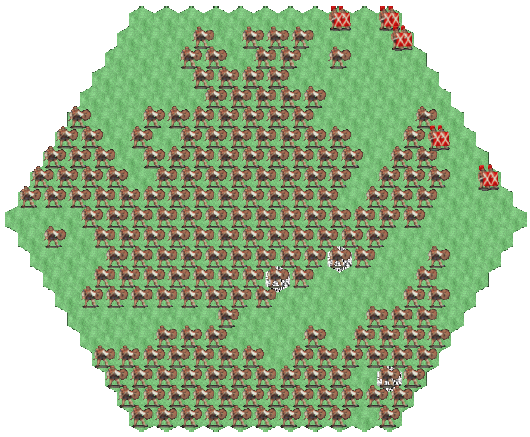
\includegraphics[width=5cm]{images/legion/before.png}
         	\begin{center}
         	Before training 
         	\end{center}
         \end{column}
         \begin{column}[T]{5cm} 
           	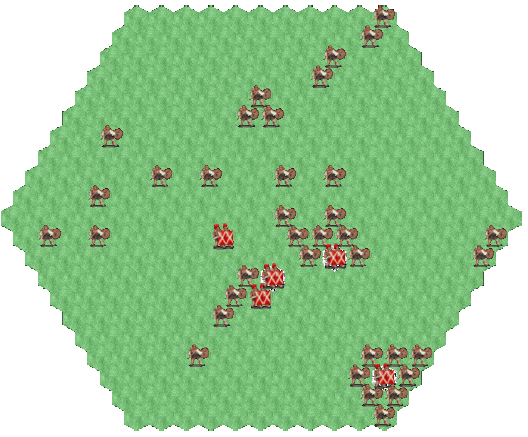
\includegraphics[width=5cm]{images/legion/after.png}
           	\begin{center}
           	After training 
           	\end{center}
         \end{column}
    \end{columns}
}

%%%%%%%%%%%%%%%%%%%%%%%%%%%%%%%%%%%%%%%%%%%%%%%%%%%%%%%%%%%%%%%%%%%%%%%%
\section{Discussions}
\frame{
    \frametitle{Questions, Suggestions or Some Other Ideas?}
}

%%%%%%%%%%%%%%%%%%%%%%%%%%%%%%%%%%%%%%%%%%%%%%%%%%%%%%%%%%%%%%%%%%%%%%%%
\section{Our Research Project}
\frame{
    \frametitle{Our Research Project}
    \begin{itemize}
        \item Motivations
        \item Mechanisms
        \item Suggestions
        \end{itemize}
}

%%%%%%%%%%%%%%%%%%%%%%%%%%%%%%%%%%%%%%%%%%%%%%%%%%%%%%%%%%%%%%%%%%%%%%%%
%%% REFERENCES
%%%%%%%%%%%%%%%%%%%%%%%%%%%%%%%%%%%%%%%%%%%%%%%%%%%%%%%%%%%%%%%%%%%%%%%%
\section{Appendix}
\setbeamertemplate{bibliography item}[book]
\frame{
    \frametitle{Further Readings: Books}
    \begin{thebibliography}{9}
        \bibitem{wooldridge2009introduction} W. Michael. {\it An introduction to
            multiagent systems}. John Wiley \& Sons, 2009.
       \bibitem{shoham2008multiagent} S. Yoav, and K. L. Brown. 
       {\it Multiagent systems: Algorithmic, game-theoretic, and logical
           foundations}. Cambridge University Press, 2008.
       \bibitem{weiss1999multiagent} W, Gerhard, ed. {\it Multiagent systems:
           a modern approach to distributed artificial intelligence}. MIT press, 1999.
   \end{thebibliography}
}
\setbeamertemplate{bibliography item}[online]
\frame{
    \frametitle{Further Readings: Courses and Labs}
    \begin{thebibliography}{9}
        \bibitem{CS224Spr} Stanford CS224M: Multi Agent Systems (Spring 2013-14). 
       \href{http://web.stanford.edu/class/cs224m/}{HERE}

        \bibitem{CPSC689} MIT CPSC689: Special Topics in Multi-Agent Systems (Spring 2006). 
       \href{http://web.stanford.edu/class/cs224m/}{HERE}
        \bibitem{StanfordGroup} Stanford Multiagent Research Group. 
       \href{http://multiagent.stanford.edu/}{HERE}
       \bibitem{AARTLab} CMU Advanced Agent-Robotics Technology Lab. 
       \href{http://www.cs.cmu.edu/~softagents/multi.html}{HERE}

       \bibitem{MITLab} MIT Robust Open Multi-Agent Systems (ROMA) Research Group. 
       \href{http://ccs.mit.edu/roma/}{HERE}
    \end{thebibliography}
}
\setbeamertemplate{bibliography item}[text]
\frame{
    \frametitle{References}
    \begin{thebibliography}{9}
        \bibitem{tan1993multi} Tan, Ming. "Multi-agent reinforcement learning:
        Independent vs. cooperative agents." {\it Proceedings of the Tenth
            International Conference on Machine Learning}. Vol. 337. 1993.
    \end{thebibliography}
}
\end{document}
